\documentclass[10pt,landscape]{article}
\usepackage{graphicx}
\usepackage{tabularx}
\usepackage{array}
\usepackage{calc}

\newlength{\seitenbreite}
\newlength{\seitenhoehe}
\newlength{\beschnittoben}
\newlength{\beschnittunten}
\newlength{\beschnittrechts}
\newlength{\beschnittlinks}
\newlength{\spinewidth}
\newlength{\totalwidth}
\newlength{\totalheight}

\setlength{\seitenbreite}{169.92mm}
\setlength{\seitenhoehe}{240mm}
\setlength{\beschnittoben}{0mm}
\setlength{\beschnittunten}{0mm}
\setlength{\beschnittrechts}{0mm}
\setlength{\beschnittlinks}{0mm} 

%%%%%%%%%%%%%%%%%%%%%%%%%%%%%%%%%%%%%%%%%%%%%%%%
% adjust this to the right size for your book
%%%%%%%%%%%%%%%%%%%%%%%%%%%%%%%%%%%%%%%%%%%%%%%%
% \setlength{\spinewidth}{2mm+.07*\pagecount}  
\setlength{\spinewidth}{20.87mm}  
%%%%%%%%%%%%%%%%%%%%%%%%%%%%%%%%%%%%%%%%%%%%%%%%%%

\setlength{\totalwidth}{\beschnittlinks+\beschnittrechts+\spinewidth+\seitenbreite+\seitenbreite}
\setlength{\totalheight}{\beschnittoben+\beschnittunten+\seitenhoehe}

\usepackage[paperheight=\totalheight%
	    ,paperwidth=\totalwidth%
	    ,left=\beschnittlinks%
	    ,right=\beschnittrechts%
	    ,top=\beschnittoben%
	    ,bottom=\beschnittunten]{geometry}

\begin{document}
\pagestyle{empty}
\setlength{\tabcolsep}{0mm}
\centering
% we use a three-column table to position the cover graphics
% I do not understand how to correctly position the spine in the center
% there must be a better way for centering the spine graphics than this
\begin{tabularx}{\totalwidth}
{p{.5\seitenbreite+.8\spinewidth}
 p{.5\seitenbreite+.20\spinewidth}
 p{\seitenbreite}}

\includegraphics{back}
& 

\includegraphics{spine} 
&
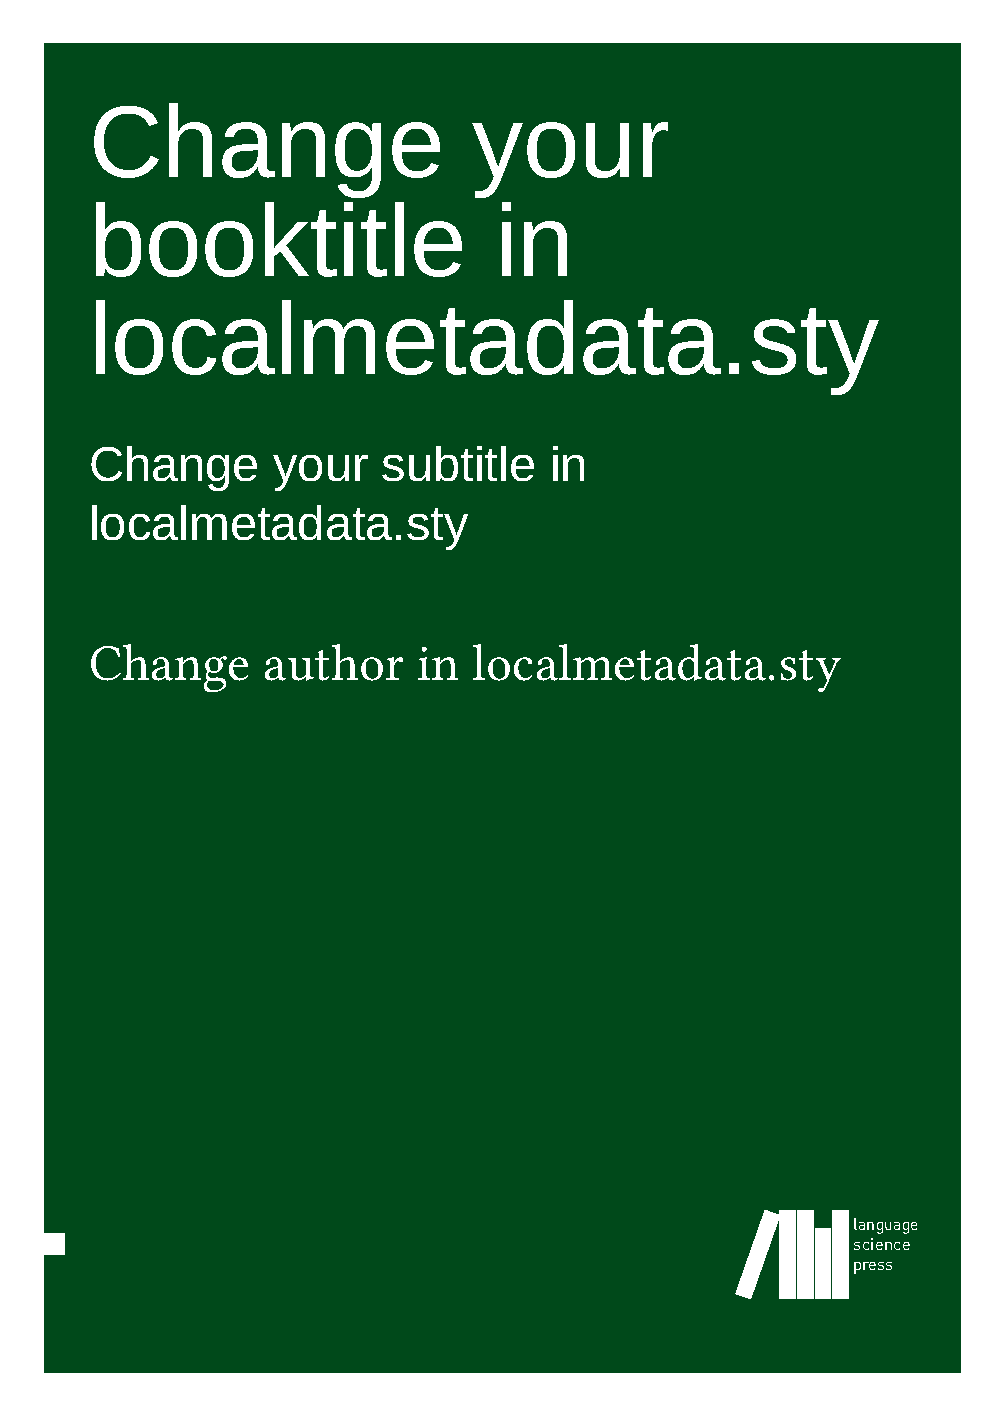
\includegraphics{front}
\end{tabularx} 

\end{document}
